\chapter{Quantum Error Correction}
Connettere tra loro più dispositivi quantistici richiede l'utilizzo di una rete quantistica. Tali collegamenti hanno un impatto fondamentale su diverse aree della Quantum Information, come:
\begin{itemize}
    \item Distribuited Quantum Computing
    \item Blind Quantum Computing
    \item Secure Classical Communication
    \item Quantum secret-sharing
    \item Molte altre applicazioni possibili
\end{itemize}

Ma questo richiede uno scambio di informazione quantistica tra i diversi dispositivi. Come visto precedentemente tale cose non è proprio facile, dato il teorema del no-cloning. Questo pone, quindi, la quantum teleportation e la quantum error correction al centro del dibattito generale. Tali tecnologie utilizzano tra di loro l'entanglement che viene "distribuito" tra i diversi dispositivi. La distribusione, fisicamente, ad oggi, avviene mediante l'utilizzo di fibre ottiche che trasportano fotoni (che possono essere entanglati anche con altre particelle). In generale la distribuzione delle coppie EPR è rumorosa (come anche nel caso classico), questo porta alla definizione dei \textbf{Canali Quantistici}.

Il modello associato ad un canale quantistico è definito a partire dalla matrice di densità \(\rho = \ket{\psi}\bra{\psi}\) del sistema che viene "elaborata" seguendo la seguente definizione:
\begin{gather*}
    \mathcal{N}(\rho) = \sum_i N_i \rho N_i^\dagger
\end{gather*}

Tale definizione può essere fatta (per il teorema di Kraus) solo se la funzione è lineare CPTP(Completamente Positivo e Traccia Preservante). L' \(\{N_i\}\) è un insieme di operatori di Kraus che soddisfano il criterio di completezza:

\begin{gather*}
    \sum_i N_i^\dagger N_i = I
\end{gather*}

Da tale definizione generale è possibile andare a definire anche il modello di Pauli del canale, dato da:
\begin{gather*}
    \mathcal{N}(\rho) = \sum_{i=0}^3p_i \sigma_i \rho \sigma_i^\dagger
\end{gather*}

Dove, \(p_i\) è la probabilità che avvenga un errore di tipo \(i\) (dove \(0\rightarrow I\), \(1 \rightarrow X\), \(2 \rightarrow Y\), \(3 \rightarrow Z\)). Le matrici \(\sigma_0 = I, \sigma_1 = X, \sigma_2=Y, \sigma_3 = Z\). Se volessimo valutare l'insieme di operatori di Kraus associati a tale modello, si avrebbe \(N_i = \sqrt{p_i}\sigma_i\). 

Dalla definizione del canale di Pauli è possibile definire anche il canale di depolarizzazione quantistica, dove, alla fine, sì ha che tutti i possibili errori di pauli sono equiprobabili, per cui il canale sarà definibile come:
\begin{gather*}
    \mathcal{N}(\rho) = (1-p)\rho + \frac{p}{3}(X \rho X^\dagger + Y \rho Y^\dagger + Z \rho Z^\dagger)
\end{gather*}

Dove la \(p\) denota la probabilità di depolarizzazione. 

Solitamente andare a studiare tali canali risulta molto oneroso, pertanto si vanno a considerare dei canali ridotti, che vanno ad isolare i singoli errori. I canali maggiormente utilizzati sono:
\begin{itemize}
    \item \textbf{Quantum Bit-Flip Channel}: \(\mathcal{N}(\rho) = (1-p)\rho + p X \rho X\)
    \item \textbf{Quantum Phase-Flip Channel}: \(\mathcal{N}(\rho)=(1-p)\rho + p Z \rho Z\)
\end{itemize}

Tali errori possono essere visualizzati mediante delle deformazioni che il canale effettua sulla sfera di Bloch stessa. L'unico valore che non viene toccato della sfera di Bloch è quello dell'errore stesso. Ad esempio nell'errore di tipo X, i valori su tale asse non cambiano. I restanti assi, invece, si contraggono di una quantità definita da \((1-2p)\). Data tale condizione, quindi, sarebbe utile andare a mappare le informazioni sull'asse che meno viene impattato dal canale, in modo da poter evitare la decoerenza. Quest'asse va a definire un sottospazio tutto suo, definito come \textbf{Decoherence Free Subspace}. Le possibili deformazioni della sfera di Bloch sono mostrate nelle figure [\ref{img:bloch-phase-flip}][\ref{img:bloch-bit-flip}][\ref{img:bloch-bit-phase-flip}]. 

\begin{figure}[H]
\centering
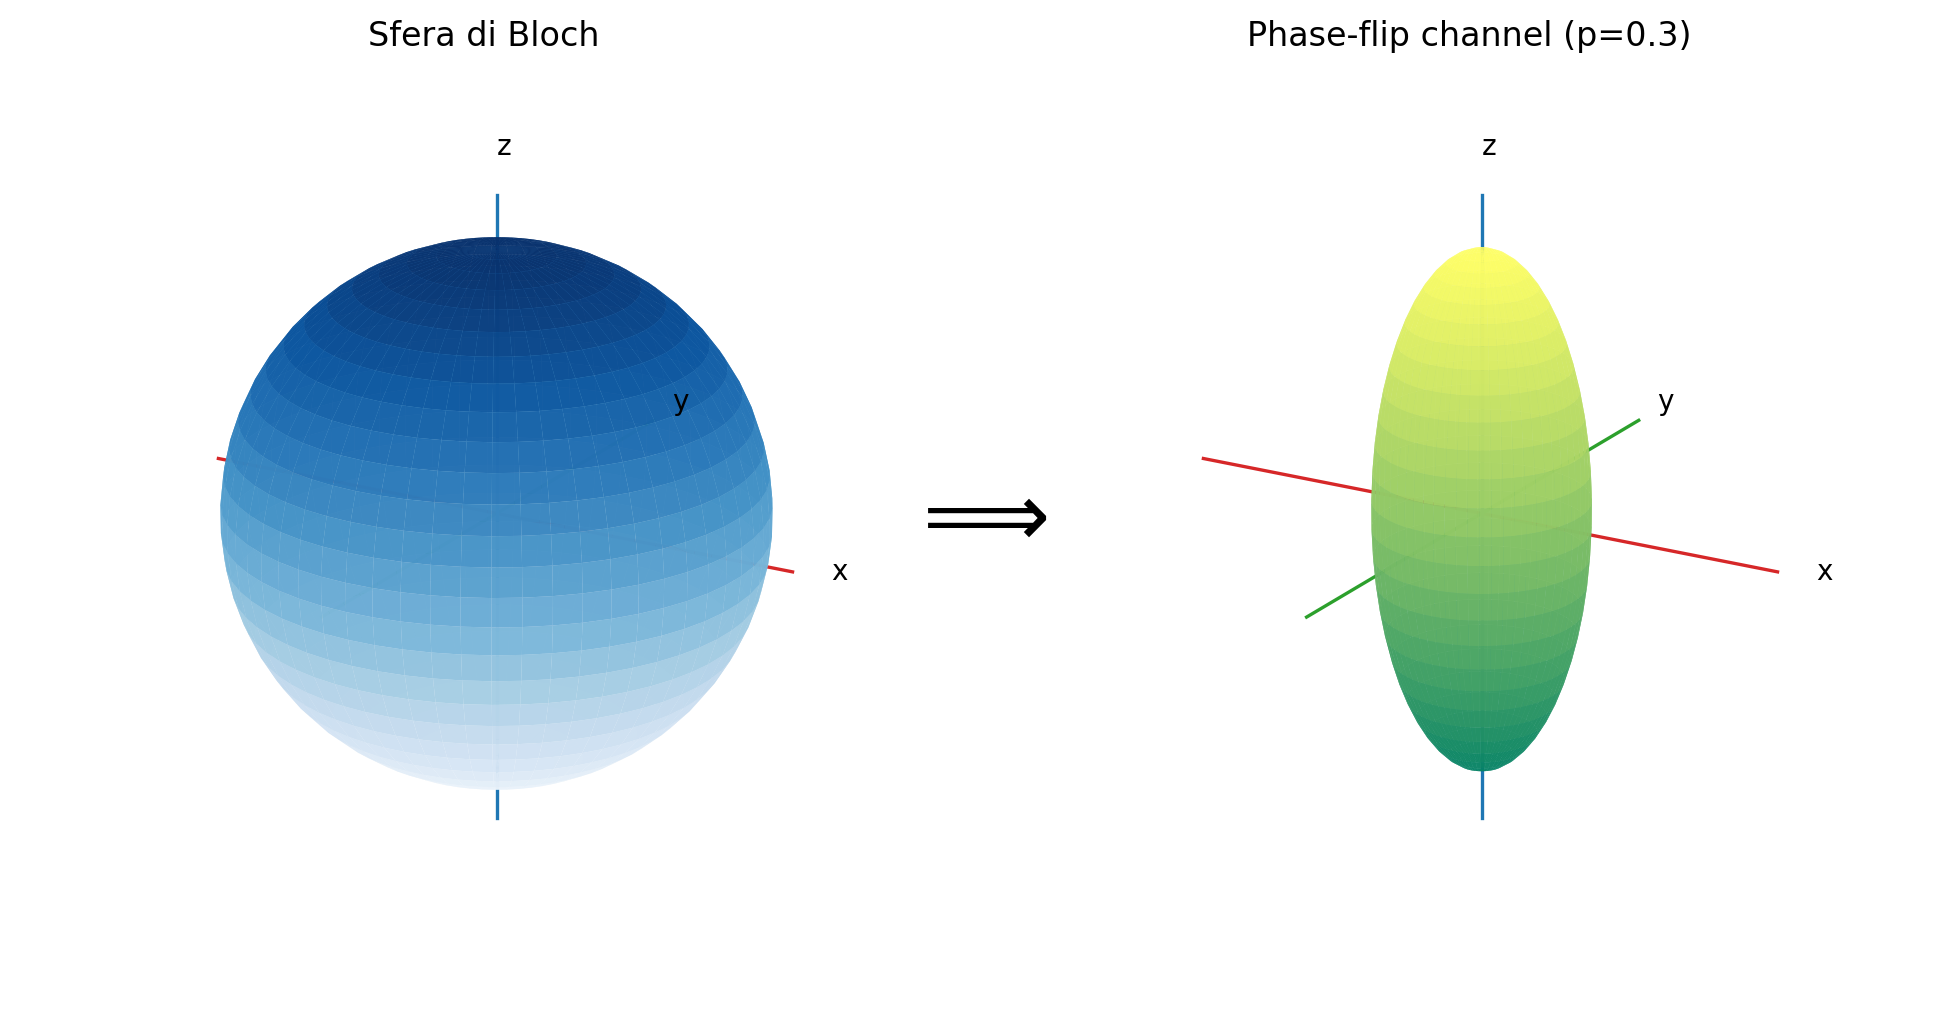
\includegraphics[width=.7\textwidth]{fig/Chapter-4/phase_flip.png}
\caption{Z Phase Flip}\label{img:bloch-phase-flip}
\end{figure}

\begin{figure}[H]
\centering
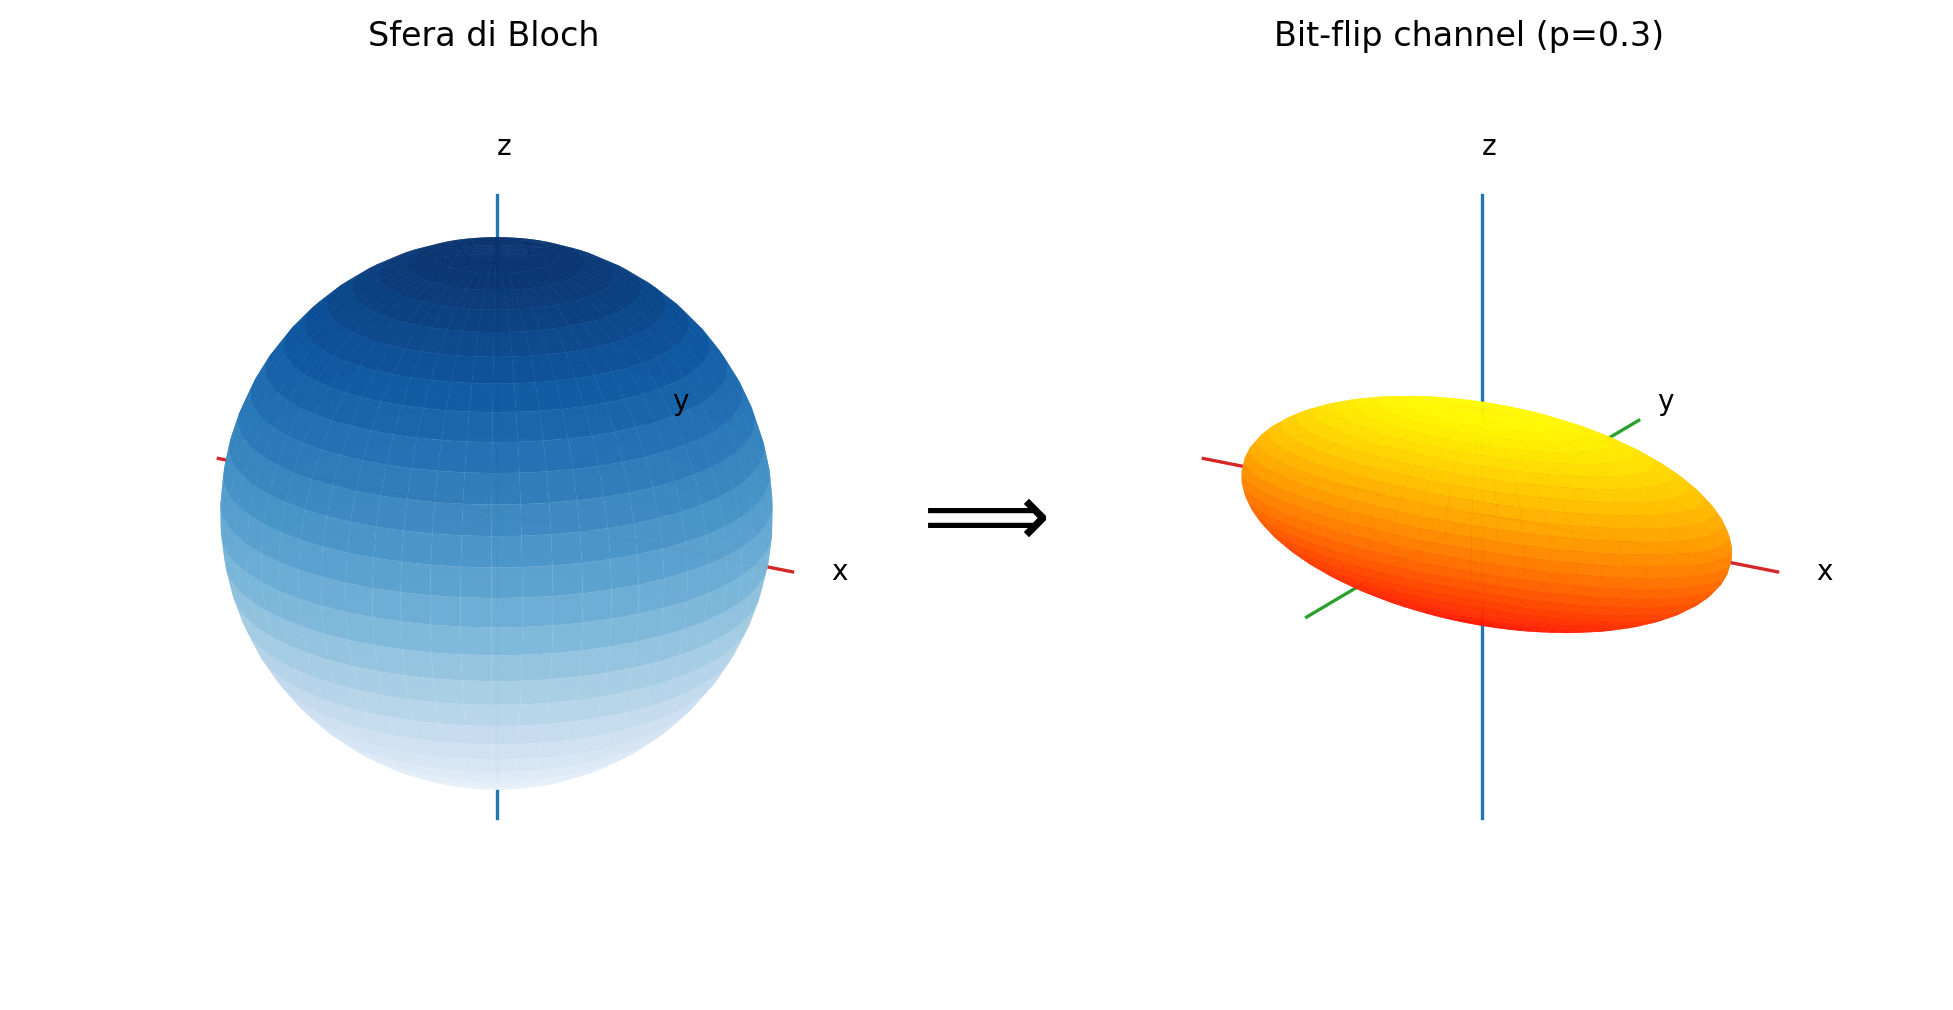
\includegraphics[width=.7\textwidth]{fig/Chapter-4/bit_flip.png}
\caption{X Bit Flip}\label{img:bloch-bit-flip}
\end{figure}

\begin{figure}[H]
\centering
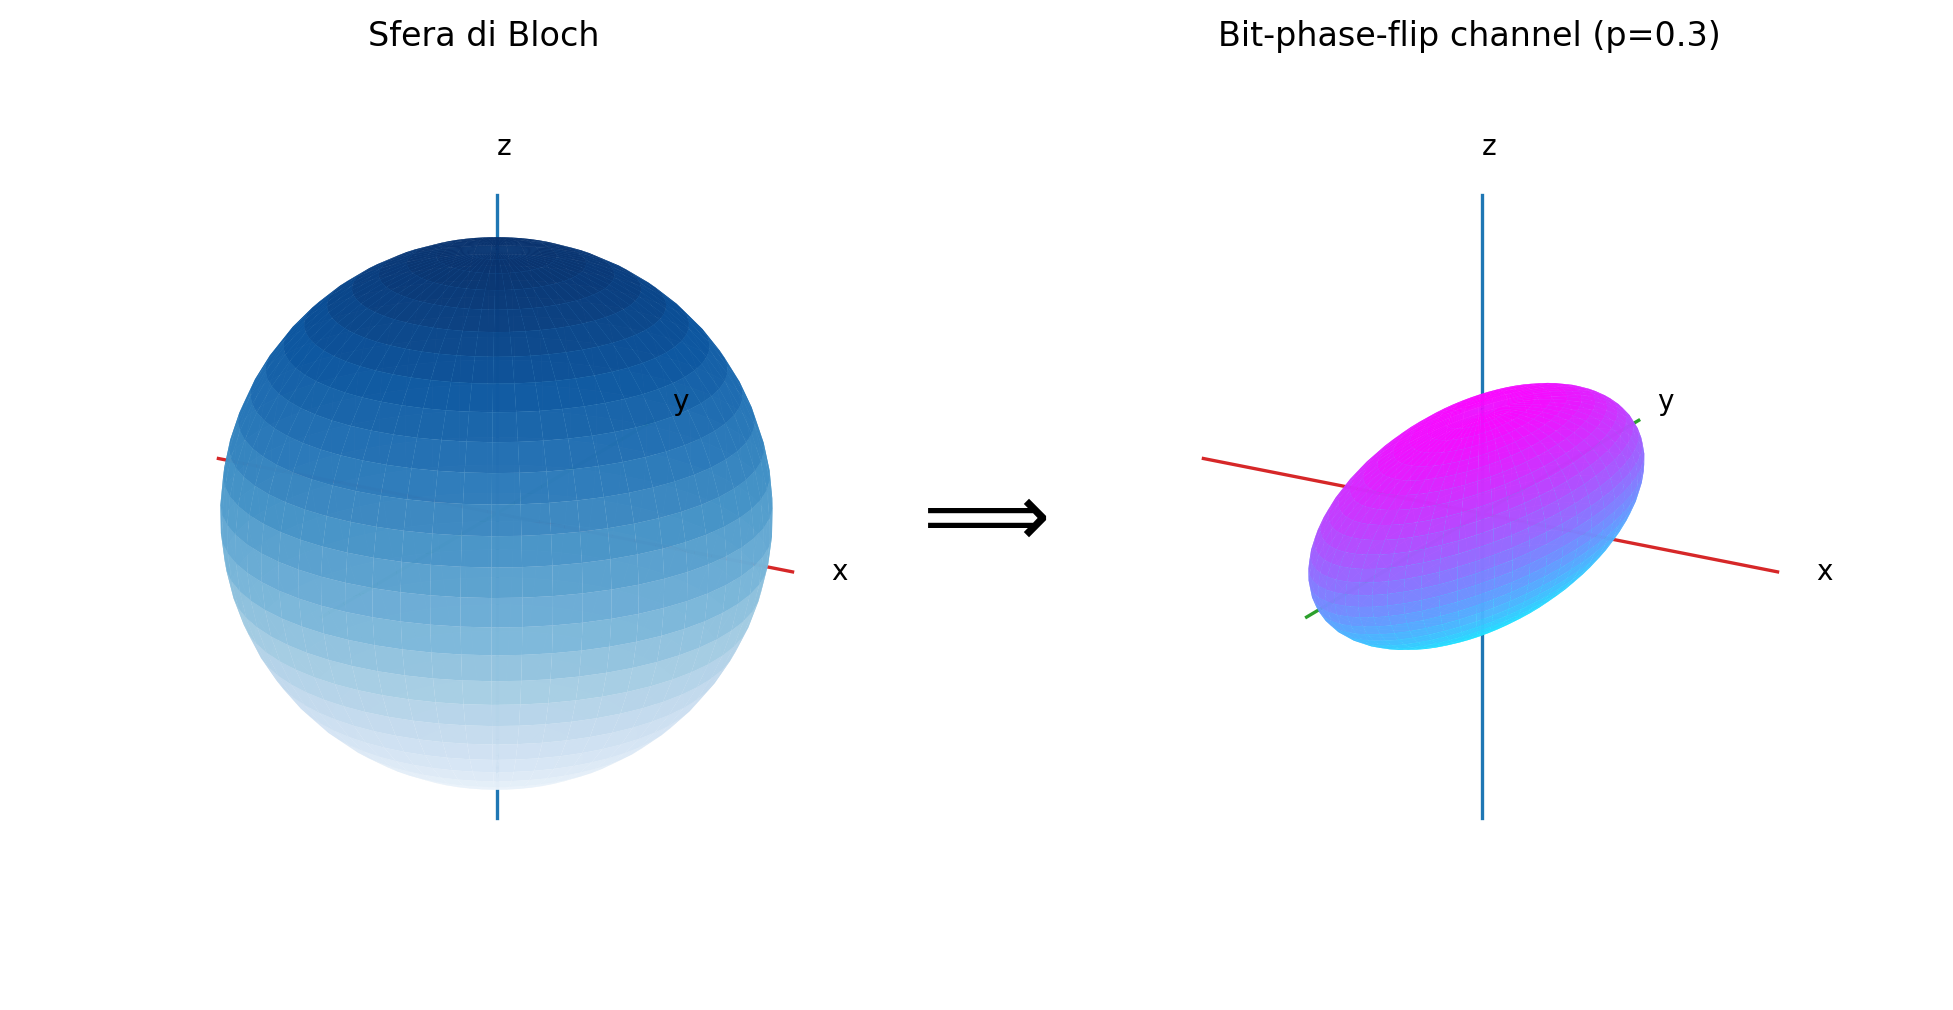
\includegraphics[width=.7\textwidth]{fig/Chapter-4/bit_phase_flip.png}
\caption{Y Pahse + Bit Flip}\label{img:bloch-bit-phase-flip}
\end{figure}

Nonostante la presenza di tali disturbi le coppie EPR rimangono coppie EPR, ma in un diverso stato di Bell. Se consideriamo come stato di partenza lo stato \(\ket{\Phi^+}_{AB} = \frac{1}{\sqrt{2}}(\ket{00}_{AB} + \ket{11}_{AB})\), avremo che, i diversi canali di Pauli presentati prima, agiranno nel seguente modo:
\begin{itemize}
    \item \textbf{Phase Flip Channel}: \(Z_A \ket{\Phi^+}_{AB} = \ket{\Phi^-}_{AB} = \frac{1}{\sqrt{2}}(\ket{00}_{AB} - \ket{11}_{AB})\)
    \item \textbf{Bit Flip Channel}: \(X_A \ket{\Phi^+}_{AB} = \ket{\Psi^+}_{AB} = \frac{1}{\sqrt{2}}(\ket{01}_{AB} + \ket{10}_{AB})\)
    \item \textbf{Y Channel}: \((XZ)_A \ket{\Phi^+} = \ket{\Psi^-}_{AB} = \frac{1}{\sqrt{2}}(\ket{01}_{AB} - \ket{10}_{AB})\)
\end{itemize}

\section{Quantum Error Correction}
Quando si parla di tecniche di error correction (che sia in caso quantistico o classico), si sta parlando di tecniche utilizzate per identificare e correggere l'errore. Nel mondo classico vi sono diverse tecniche che permettono di fare \textbf{error detection}(detectare l'errore) ed \textbf{error correction}. Una di queste è il codice a ripetizione che è stato esteso anche al caso quantistico. Pertanto gli si da una breve paronamica.

\subsection{Codice a ripetizione}
Dato un canale rumoroso, nel mondo classico, quello che può accadere è il fenomeno del bit flip. Quindi un bit quando viene inviato, al ricevitore, viene flippato dal canale stesso. Quindi da 0 diventa 1 o il vicevera.
Per modellare un sistema che permetta di essere "resistente" al canale si è pensato di poter replicare l'informazione più volte in modo che il ricevitore, anche nel caso di qualche bit flip, possa riconoscere l'informazione originale. Dalla teoria dell'informazione si dice che è possibile arrivare ad una probabilità di errore piccola a picere andando ad aumentare il numero di repliche dell'informazione (tale tecnica viene anche da una nostra predisposizione naturale, quando qualcuno non capisce qualcosa che gli stiamo dicendo, tendiamo a ripeterla più volte). Una delle tecniche più semplici è il \textbf{codice a ripetizione}. Un codice a ripetizione è un codice che va ad aumentare il numero di bit inviati per la singola informazione. Per esempio, se voglio inviare 0, lo invierò 3 volte (\(0 \rightarrow 000\)), lo stesso per 1 (\(\ \rightarrow 111\)). Con tale codice, il ricevitore utilizzerà un sistema di votazione per capire l'informazione inviata. Se su 3 bit vi è una maggioranza i 0, allora tale bit sarà considerato come 0. Lo stesso vale per gli 1.

In generale, considerando un \textbf{canale simmetrico}(dove le probabilità di flip di 1 e 0 sono uguali), la cui probabilità di flip è \(p\) è facile andare a valutare il caso in cui il ricevitore riceverà la risposta sbagliata se si avranno 2 o 3 errori all'interno del codice (nel caso di 3 ripetizioni). Quindi valutando le diverse combinazioni di errore che si possono avere si avrà che la probabilità di errore si calcolerà come: \(P_e = 2 p^2 (1 - p) + p^3\) dove il primo termine racchiude le 3 combinazioni possibili nel caso di 2 errori, mentre l'ultimo termine racchiude il caso singolo di 3 errori (tali casi sono gli unici in cui il ricevitore non riesce a raggiungere l'informazione corretta). Facendo due calcoli, quindi, si raggiunge che la probabilità di errore per un codice a 3 bit è \(P_e = 3 p^2 - 2 p^3\).

\subsection{"Codici a ripetizione" Quantistici}
Il caso classico non è direttamente estendibile al caso quantistico, questo è dovuto al fatto che ci sono fenomeni come il no-cloning, il collasso del qubit dopo una misura ed i diversi tipi di errori a cui il qubit va incontro (\(X,Y,Z\)). Per cercare di compensare questa cosa, allora, si è cercato un modo per poter "estendere" l'informazione su più qubit. Questo andando ad utilizzare degli stati entanglati tra di loro (da cui la famosa fase: "Combattiamo l'entanglement con l'entanglement" di Preskill). Per comprendere al meglio il funzionamento di tale tecnica, andiamo a considerare uno stato quantistico:
\begin{gather*}
    \ket{\psi} = \alpha \ket{0} + \beta \ket{1}
\end{gather*}

Andando a "spalmare" l'informazione su più qubit mediante le CNot si ottiene:
\begin{align*}
    \ket{\psi} &= \alpha \ket{000} + \beta \ket{111}\\
               &= \alpha \ket{0_L} + \beta \ket{1_L}
\end{align*}

Da tale relazione riusciamo anche a notare la definizione del \textbf{Qubit Logico}(\(\ket{0_L}\) e \(\ket{1_L}\)). Rispetto al caso classico non è proprio una replica vera e propria dell'informazione, purtroppo per il problema del no-cloning si avrà sempre che un qubit non può essere replicato in alcun modo. Però almeno l'informazione viene espressa su più qubit. Tale sistema, andando ad utilizzare ulteriori due qubit, permette di fare error detection e capire su quale qubit il canale abbia effettuato un "bit-flip" (X-Noise). Per comprendere al meglio il funzionamento di tale sistema si presenta lo schema nell'immagine [\ref{img:error-correction-codes}]

\begin{figure}[H]
\centering
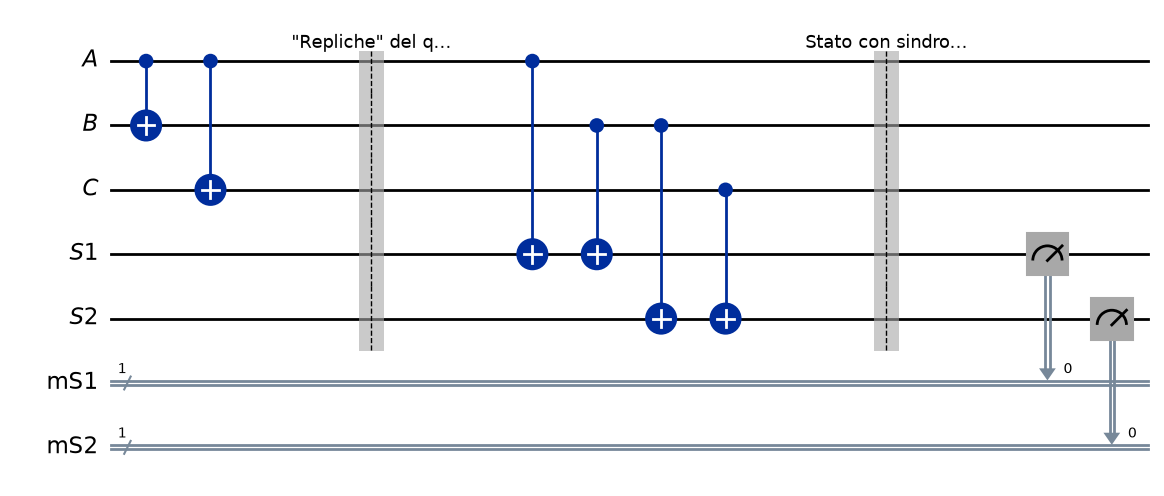
\includegraphics[width=.9\textwidth]{fig/Chapter-4/quantum.ecc-scheme.png}
\caption{Informazione codificata su più qubit}\label{img:error-correction-codes}
\end{figure}

Per fare due conti, lo stato iniziale è il seguente:
\begin{gather*}
    \ket{psi} = \ket{\phi_A} \otimes \ket{0_B} \otimes \ket{0_C}
\end{gather*}
Andando a considerare che \(\ket{\phi_A} = \alpha \ket{0} + \beta \ket{1}\), si avrà:
\begin{align*}
    \ket{\psi} &= \ket{\phi_A} \otimes \ket{0_B} \otimes \ket{0_C}\\
    &= (\alpha \ket{0} + \beta \ket{1}) \otimes \ket{0_B} \otimes \ket{0_C}\\
    &= \alpha \ket{0_A 0_B 0_C} + \beta \ket{1_A 0_B 0_C}
\end{align*}

Andando ad effettuara le due C-Not, i due termini finali nel secondo elemento dell'equazione passano da 0 ad 1, diventando:
\begin{align*}
    \ket{\psi} &= \alpha \ket{0_A 0_B 0_C} + \beta \ket{1_A 1_B 1_C}
\end{align*}

Ottenendo i qubitlogici. Se si fanno passare per un canale di tipo X-Noise, si avrà che, considerando un solo possibile errore, che gli stati saranno:
\begin{align*}
    \ket{\psi} &= \alpha \ket{100} + \beta \ket{011}\\
    \ket{\psi} &= \alpha \ket{010} + \beta \ket{101}\\
    \ket{\psi} &= \alpha \ket{001} + \beta \ket{110}
\end{align*}

Definiti tali casi di errore, si va a considerare che, effettuando le interazioni con le ancille, si avrà che:
\begin{itemize}
    \item \(\ket{0_{S1} 0_{S2}}\): Non c'è alcun tipo di errore
    \item \(\ket{0_{S1} 1_{S2}}\): Vi è un errore sul terzo qubit (di tipo X-Noise)
    \item \(\ket{1_{S1} 0_{S2}}\): Vi è un errore sul primo qubit
    \item \(\ket{1_{S1} 1_{S2}}\): Vi è un errore sul secondo qubit
\end{itemize}

La misura mediante le ancille permette di non perturbare in alcun modo lo stato cercando di estrarre informazioni solo su eventuali cambiamenti avvenuti ai qubit. Questo seguendo la seconda parte dello schema visualizzabile alla figura [\ref{img:error-correction-codes}]. Da tale schema è possibile immaginare anche un eventuale controllo che va a pilotare una porta X controllata da bit classici. Effettuata la detection dell'errore questo viene corretto prima della detection. Lo schema del decodificatore si visualizza all'immagine [\ref{img:quantum-decoder}].

\begin{figure}[H]
\centering
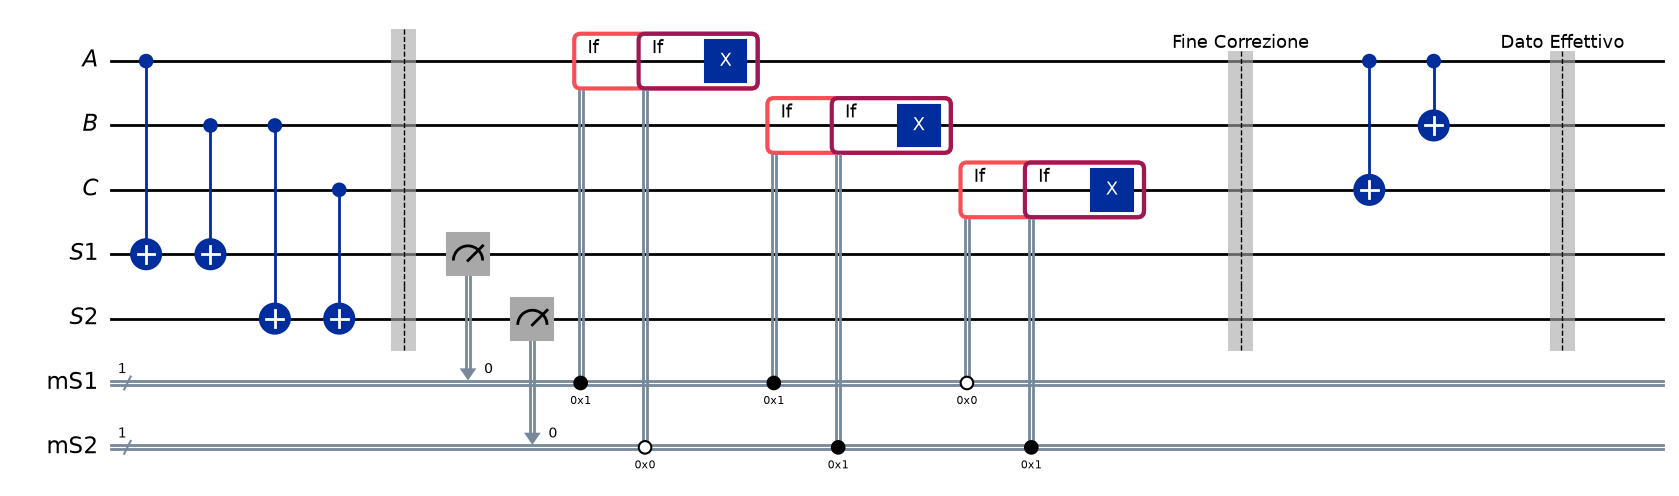
\includegraphics[width=\textwidth]{fig/Chapter-4/decoding.png}
\caption{Quantum Error Correction and Decoding}\label{img:quantum-decoder}
\end{figure}

Alla fine del circuito [\ref{img:quantum-decoder}] il primo qubit sarà esattamente il qubit che si è voluto inviare, questo a meno di al più un errore di bit flip sul dato inviato. Nonostante stiamo parlando di comunicazioni tali sistemi si vanno ad utilizzare anche su delle strutture fisiche locali. Un esempio di applicazione di tali sistemi sono i surface-code, che vanno ad utilizzare in maniera morbosa tale sistema.




